\documentclass{article}
\usepackage{lmodern}
\usepackage[font=small,labelfont=bf]{caption}
\usepackage{mathrsfs}
\usepackage[utf8]{inputenc}
\usepackage{amsmath, fge}
\usepackage[amsmath,thmmarks]{ntheorem}
\usepackage{amssymb}
\usepackage{amsthm}
\usepackage[margin=1in]{geometry}
\usepackage{amsfonts}
\usepackage{upgreek}
\usepackage{dashbox}
\usepackage[bottom]{footmisc}
\usepackage{pdfpages}
\usepackage{graphicx}

\usepackage{mathtools}
\newlength{\temp}
\usepackage{siunitx}
\usepackage{hyperref}
\usepackage{enumitem}
\usepackage{amsbsy}
\hypersetup{
    colorlinks=true,
    linkcolor=blue,
    filecolor=magenta,      
    urlcolor=cyan,
    pdftitle={Overleaf Example},
    pdfpagemode=FullScreen,
    }
\usepackage{babel}
\usepackage{mleftright,mathtools}
\usepackage{bm}
\usepackage{fancyhdr}
\pagestyle{fancy}
\lhead{Ahou L. -  Ahou S. - Fiorini L. - Portier A.} % controls the left corner of the header
\chead{} % controls the center of the header
\rhead{Groupe 49} % controls the right corner of the header
\lfoot{} % controls the left corner of the footer
\cfoot{} % controls the center of the footer
\cfoot{~\thepage} % controls the right corner of the footer
\usepackage{titlesec}



\begin{document}


%\pagestyle{fancy}
\thispagestyle{empty}
\begin{titlepage}
	\begin{center}
		\begin{figure}
			\raisebox{-0.5\height}{
\includegraphics[width=.35\textwidth]{logo_ucl.png}}\hfill
			\raisebox{-0.5\height}{
\includegraphics[width=.1\textwidth]{logo_epl.png}}
        \end{figure}
		
		\textsc{\LARGE École Polytechnique de Louvain\\faculté de l'Université catholique de Louvain}\\[1cm]

		\textsc{\large LINMA1702 - Modèles et méthodes d'optimisation I}\\[0.5cm]
		\textsc{\large Année académique 2023 -- 2024}\\[0.5cm]

		% Title
		\HRule \\[0.4cm]
		{ \huge \bfseries Rapport : 1\textsuperscript{ère} partie\\[0.4cm] }
		\HRule \\[0.75cm]

		% Author and supervisor
		
\begin{minipage}{0.4\textwidth}
\begin{flushleft}
\Large
Groupe 49:\\
\textsc{Ahou} Lucas\\
\textsc{Ahou}  Samuel \\
\textsc{Fiorini} Lucien \\
\textsc{Portier}  Adrien \\

\end{flushleft}
\end{minipage}
\begin{minipage}{0.4\textwidth}
\begin{flushright}
\Large
NOMA:\\
3594-22-00\\
4408-19-00\\
7502-22-00 \\
5337-22-00\\
\end{flushright}
\end{minipage}


\\ [2 cm]
\Large
Professeur:\\
\textsc{Glineur} François\\

		
		\vfill
		%\begin {center}
		%    \includegraphics[width=0.45\textwidth]{img/couv1}
		%\end{center}
		
		\vfill
		
		% Bottom of the page
		{\large Avril 2024}
		
		\newpage
		%\thispagestyle{empty}

		\setcounter{tocdepth}{3}
		\vfill
	\end{center}
\end{titlepage}
%-----------------------------------------------------------
% début du document numéroté
\clearpage
\pagenumbering{arabic}

\section*{Question 1}

\subsection*{A.}
\subsubsection*{Modélisation du problème}
Afin de garantir que le niveau de production ne soit pas trop bas, il nous a été demandé de maximiser le niveau minimal de production au cours de l'année. Nous allons discuter dans cette section de notre choix de modélisation pour ce problème.\\
Vous trouverez ci-dessous une table regroupant les notations utilisées dans notre modèle \footnote{Bien que $n$ et $m$ soient des constantes, nous utilisons ces notations pour alléger les formules et également pour rester dans un cadre général. Tout autre paramètre/variable sera introduit lorsque cela sera nécessaire.}:
\begin{table}[h!]
\centering
\renewcommand{\arraystretch}{1.5}% Add spacing between rows : default value is 1
\begin{tabular}{|c || c |} 
 \hline
Nom & Signification\\
 \hline\hline
 $P$  & Puissance totale à installer\\
 $\kappa \in [0, 1]$ & Proportion de la puissance totale à installer en sites \textit{offshore}\\
 $c^\text{max}_i$ & Capacité maximale installable pour le i\textsuperscript{ème} site\\
 $c_i \in [0, c_i^{\max}]$ & Capacité effectivement installée sur le i\textsuperscript{ème} site\\
 $e_i(t) \in [0,1]$ & Rendement du i\textsuperscript{ème} site au temps $t$\\
 $n$ & Nombre de sites\\
 $m$ & Nombre d'heures dans une année\\
 \hline
\end{tabular}
\caption{Table des notations utilisées pour le modèle}
\label{table:noms_des_variables}
\end{table}
\noindent \\
Parmi toutes ces variables, ce sont les $c_i$ que nous cherchons à optimiser. L'idée derrière notre choix de modèle est la suivante : \\
Pour toutes les heures de l'année, nous prenons la somme de production de tous les sites en tenant compte du choix des $c_i$. Nous obtenons ainsi une fonction de la production totale en fonction du temps et dont l'allure dépend du choix des $c_i$.
Un tableau illustratif est repris ci-dessous :
\begin{table}[h!]
\centering
    \[ \begin{array}{c|cccc}
      t_i    & {t_0} & {t_1} & {\ldots}  & {t_{m-1}}\\
      \hline
      e_0(t_i) & 0.25       & 0.08   &\ldots    & 0.17 \\
      e_1(t_i) & 0.87       & 0.69   &\ldots    & 0.42 \\
      \vdots   & \vdots     & \vdots  &\vdots   & \vdots \\
      e_{n-1}(t_i) & 0.15       & 0.207   &\ldots    & 0.94 \\
      \hline
      \text{Prod. totale} &\scriptstyle \sum \limits_{i=0}^{n-1}c_i e_i(t_0) &\ldots &\ldots &\scriptstyle \sum \limits_{i=0}^{n-1}c_i e_i(t_{m-1})\\
    \end{array} \]
\caption{Table représentant les valeurs de rendement de chaque site ainsi que la production totale en fonction du temps (à titre illustratif).}
\label{table:table_rendement_illustratif}
\end{table}
\newpage
Nous cherchons donc à maximiser la valeur minimale de la production totale. Avec toutes ces informations, nous pouvons écrire notre modèle :
\begin{align*}
    \max_{c_i} \quad  
    \min_t \{ &\sum_{i=0}^{n-1}c_i e_i(t) \} \\ 
    \sum_{i=0}^{n-1} c_i &= P\\
    \sum_{\text{\tiny offshore}}c_i &= \kappa P\\
    0 &\le \, c_i \, \le c_i^{\max}\\
\end{align*}
Cependant, celui-ci n'est pas linéaire à cause de la fonction $\min$. Nous introduisons alors une variable intermédiaire $\gamma$ afin de remplacer le $\min$ par un problème de maximisation comme vu au cours. Le nouveau modèle, maintenant linéaire, s'écrit comme suit \footnote{La contrainte imposant que la variable $\gamma$ soit positive n'est pas nécessaire car le minimum est strictement positif et que $\gamma$ prendra cette valeur.} :
\begin{align}
    \max_{c_i, \gamma} \quad &\gamma \nonumber \\ 
    \sum_{i=0}^{n-1} c_i &= P\\
    \sum_{\text{\tiny offshore}}c_i &= \kappa P\\
    \gamma &\le \sum_{i=0}^{n-1} c_i e_i(t_j) \quad \forall j \in \{0, \ldots, m-1\}\\
    0 &\le \, c_i \, \le c_i^{\max} \quad \forall i \in \{0, \ldots, n-1\}
\end{align}
La contrainte (1) représente la puissance totale qu'il faut installer en Europe. La contrainte (2) indique qu'il faut exactement une proportion $\kappa$ de la puissance $P$ installée en \textit{offshore}. La contrainte (3) dit que la variable intermédiaire $\gamma$ ne doit pas dépasser la valeur du minimum de la fonction de production totale. Enfin, la contrainte (4) indique les bornes sur les variables $c_i$

\subsubsection*{Estimation de la taille du modèle}
\noindent
Au total, nous avons $\overbrace{n}^{c_i} + \overbrace{1}^{\gamma}$
variables et $\overbrace{m}^{\text{(3)}} + \overbrace{2}^{\text{(1) \& (2)}}$ contraintes \textbf{en plus} des bornes sur les $c_i$.\\
Cependant, lors de la résolution le \textit{solver} traduit le problème sous forme standard. Ainsi, il introduit $n + m$ variables de \textit{slack} qui correspondent au contraintes (3) et (4). Nous nous retrouvons alors avec le problème suivant : 
\begin{align*}
    \max_{c_i, \gamma} \quad  
    &\gamma \nonumber \\ 
    \sum_{i=0}^{n-1} c_i &= P\\
    \sum_{\text{\tiny offshore}}c_i &= \kappa P\\
    \gamma + s_j &= \sum_{i=0}^{n-1} c_i e_i(t_j) \quad \forall j \in \{0, \ldots, m-1\}\\
    c_i + t_i &\le c_i^{\max} \quad \forall i \in \{0, \ldots, n-1\}\\
    c_i, \gamma, s_j, t_i &\ge 0
\end{align*}
Ce qui mène à un total de $2n + m + 1$ variables et $m + n + 2$ contraintes.

\subsection*{B.}
Pour résoudre le modèle décrit dans la section précédente, nous avons utilisé la fonction \verb|linprog| de la librairie \verb|SciPy|.\\
La solution retournée par le solver pour les paramètres $P = 500000 [\mathrm{MW}]$ et $\kappa = 0.17$ nous indique qu'il y a $267$ sites sur lesquels la puissance installée est non nulle, ce qui veut dire qu'il y a $642 - 267 = 375$ sites sur lesquels il est préférable de ne pas installer d'éoliennes.\\
La répartition de puissance est représentée sur la carte ci-dessous \footnote{Les croix représentent les sites sur lesquels la puissance installée est nulle.} :

\begin{figure}[h!]
    \centering
    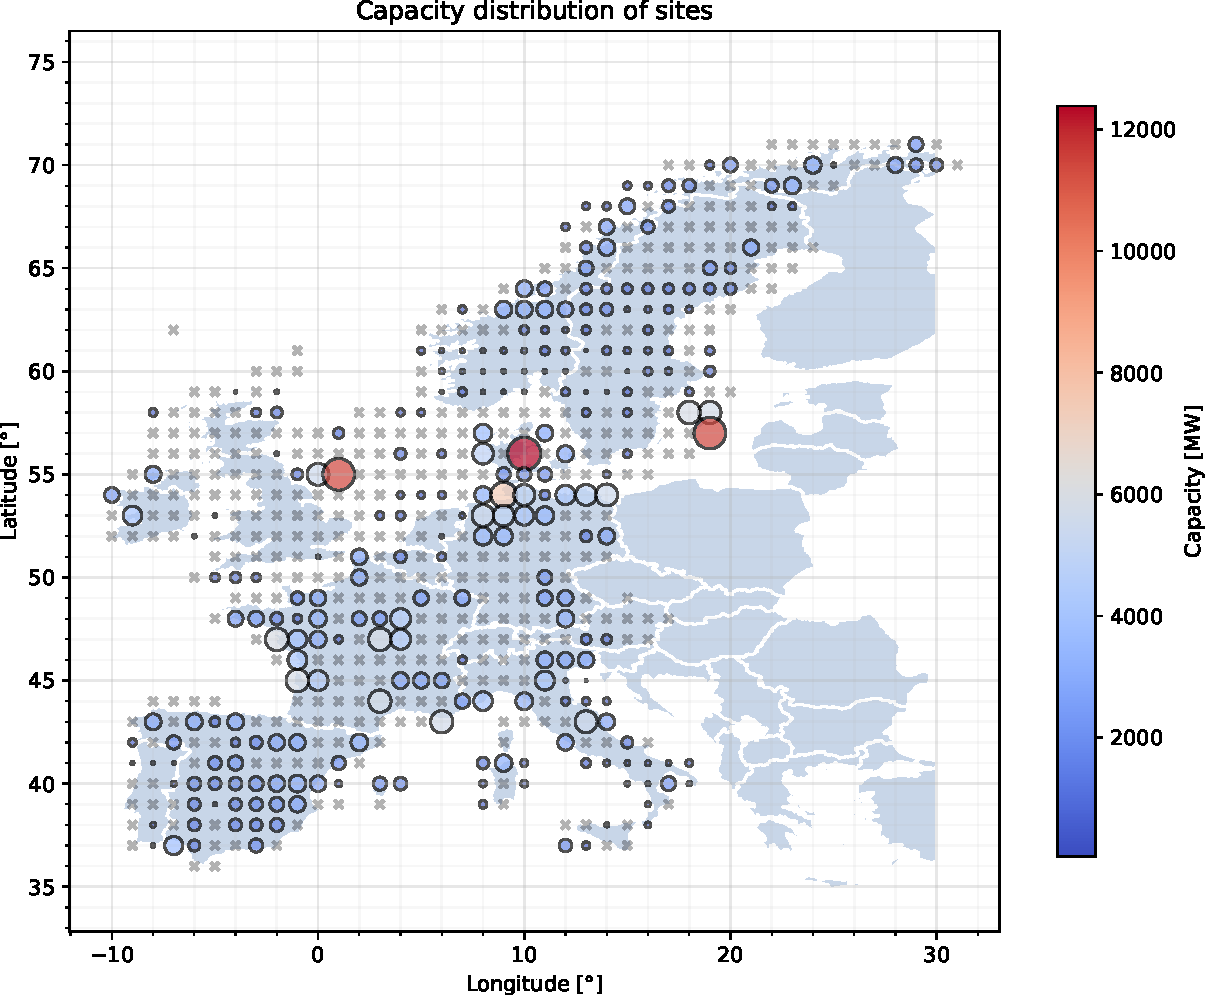
\includegraphics[scale=0.5]{Images/Partie_1/Q1/capacity_distribution.pdf}
    \caption{Carte représentant la répartition de puissance sur les différents sites d'éoliennes}
    \label{fig:capacity_distribution_partie1}
\end{figure}

\newpage

Quant au temps de résolution du solver, celui-ci prend en moyenne $1.825 [\mathrm{s}]$ pour renvoyer une solution. Un graphe des performances est représenté ci-dessous :

\begin{figure}[h!]
    \centering
    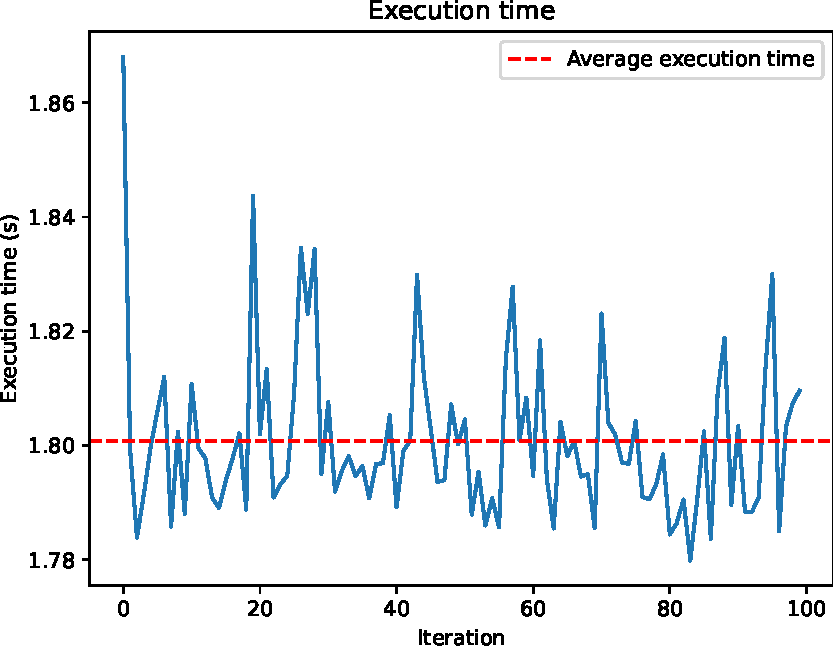
\includegraphics[scale=0.5]{Images/Partie_1/Q1/execution_time.pdf}
    \caption{Graphe du temps d'exécution sur 100 itérations}
    \label{fig:execution_time_partie1}
\end{figure}

Nous pouvons également nous intéresser à l'énergie totale produite sur l'année ainsi que sur chaque période d'une heure.
En prenant compte des rendements qui nous ont été fournis et en utilisant la solution obtenue par le solver,
il est possible de calculer, en chaque heure, l'énergie produite. Le graphe représentant la production d'énergie en fonction du temps est représenté ci-dessous :

\begin{figure}[h!]
    \centering
    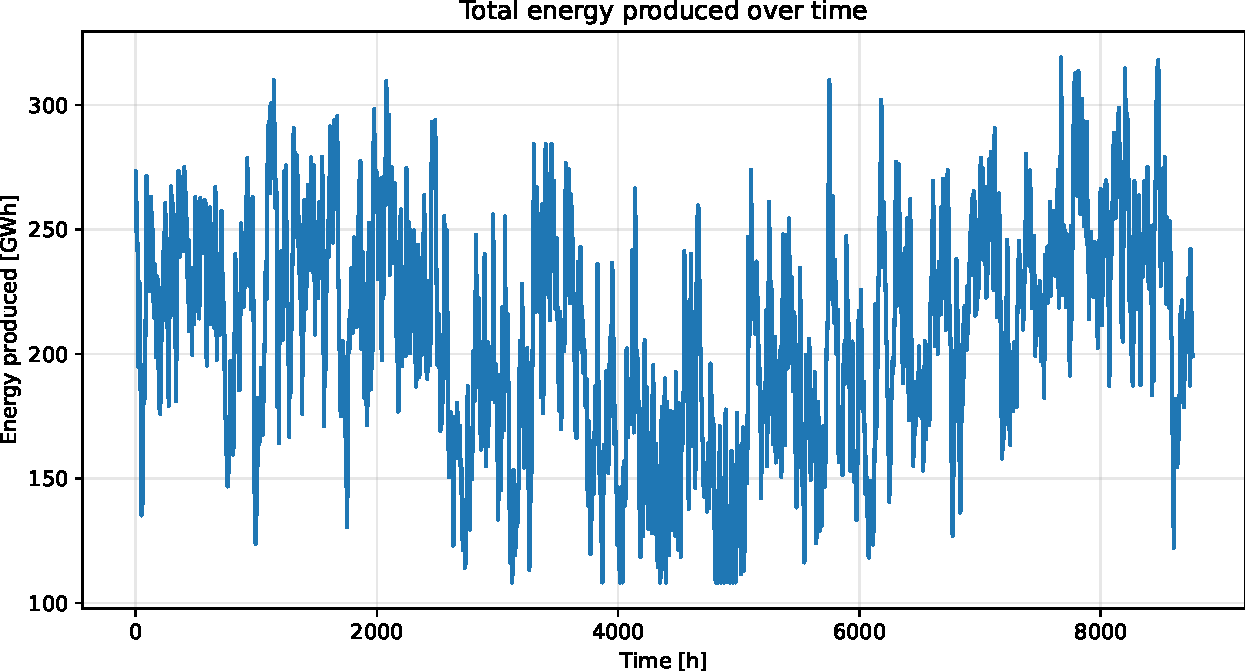
\includegraphics[scale=0.5]{Images/Partie_1/Q1/energy_produced.pdf}
    \caption{Graphe de la production d'énergie en fonction du temps}
    \label{fig:energy_produced_partie1}
\end{figure}
Et en sommant toutes les productions, nous obtenons une valeur d'environ $1828762.56 [\mathrm{GWh}]$. 
\newpage
Nous pouvons, de manière similaire, calculer le rendement de production simplement en divisant la production sur une heure par la production idéale (i.e. $P*1\mathrm{h} = P [\mathrm{MWh}]$).\\
Nous obtenons alors le graphe suivant où nous pouvons observer une moyenne de $42\%$ de rendement :

\begin{figure}[h!]
    \centering
    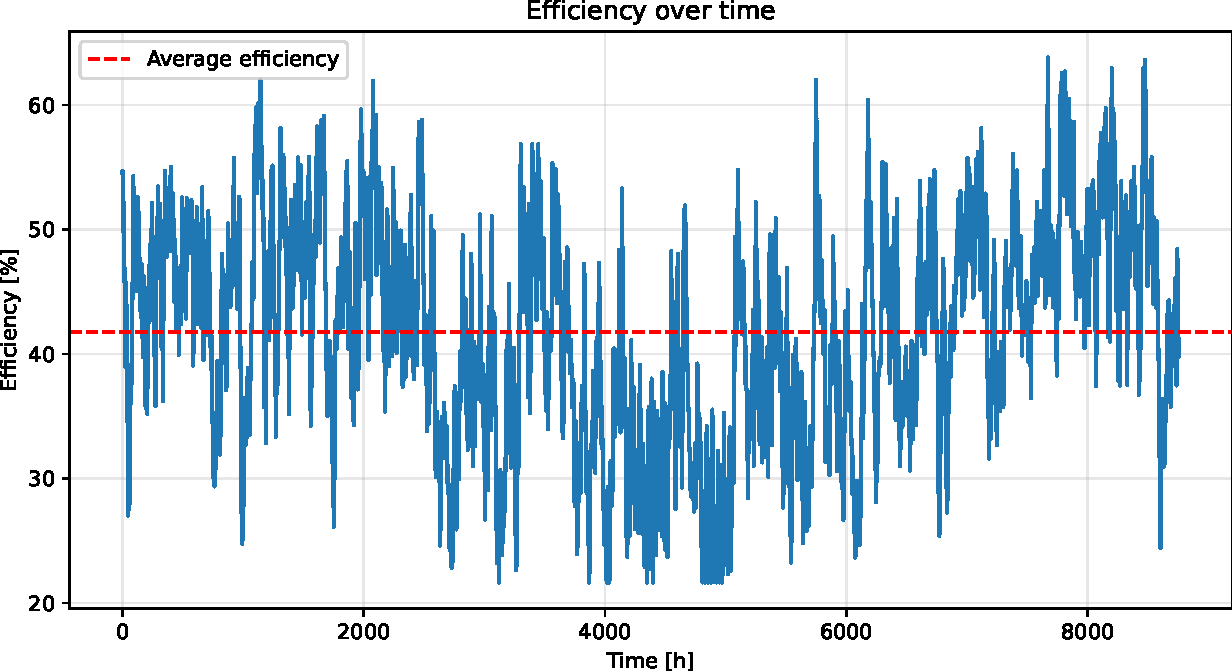
\includegraphics[scale=0.5]{Images/Partie_1/Q1/efficiency.pdf}
    \caption{Graphe du rendement de production en fonction du temps}
    \label{fig:efficiency_partie1}
\end{figure}

\subsection*{C.}
\subsubsection*{(a)}
Nous avons vu au cours que les variables du problème dual associé au primal permettent de calculer la variation de la fonction objectif
lorsque l'on modifie la valeur d'une des contraintes. Lorsque l'on change la valeur de la puissance maximale installable de $P$ à $\Delta P$, la variable $y_1$ du problème dual nous indiquera de combien change
la fonction objectif (i.e. la valeur de production minimale). Nous avons donc :
\begin{equation*}
    \Delta \gamma = y_1 \Delta P
\end{equation*}

\subsubsection*{(b)}
Pour déterminer les sites les plus rentables sur lesquels on augmenterait la capacité dans le cas d'une modification de la puissance maximale installable, il suffit de regarder les variables duales associées aux contraintes de capacité maximale installable. En effet, ces variables nous indiquent de combien la fonction objectif varie lorsque l'on modifie la capacité maximale installable d'un site.
Nous pouvons donc résoudre le problème dual associé au primal pour obtenir ces valeurs. Après résolution, nous obtenons que les dix sites les plus intéressants sont les sites $\{241, 296, 311, 312, 313, 314, 315, 330, 434, 437\}$.\\
Cependant, lorsque nous regardons les sites où le rendement moyen est maximal, nous obtenons : $$\{ 69, 166, 167, 235, 236, 237, 434, 447, 525, 623 \}$$
Nous voyons donc que, sauf exception, il n'y pas de lien entre les sites les plus rentables quant à l'augmentation de la puissance installable et ceux où le rendement est maximal.
\newpage

\section*{Question 2}

\subsection*{A.}
Dans cette deuxième question, nous avons maintenant la possibilité
d'acheter de l'énergie en chaque heure en plus de l'énergie produite par les éoliennes.
Toutefois, nous pouvons acheter qu'une quantité maximale $E_{\text{max}}$ d'énergie.\\

\subsubsection*{Modélisation du nouveau problème}
Pour représenter l'achat d'énergie en chaque heure de l'année, nous pouvons introduire $m$ nouvelles variables $a_j$ pour $j \in \{ 0, \ldots, m-1 \}$.\\
Notre nouveau vecteur de variables de décisions devient alors : 
\[ \bm{x} = (c_0, \ldots, c_{n-1}, a_0, \ldots, a_{m-1}, \gamma )^\intercal \]
Et notre nouveau problème devient donc :
\begin{align*}
    \max_{c_i, a_j, \gamma} \quad  &\gamma \\ 
    \sum_{i=0}^{n-1} c_i &= P\\
    \sum_{\text{\tiny offshore}}c_i &= \kappa P\\
    \gamma &\le \sum_{i=0}^{n-1} c_i e_i(t_j) + a_j \quad \forall j \in \{0, \ldots, m-1\}\\
    \sum _{j=0}^{m-1} a_j &\le E_{\text{max}}\\
    0 &\le \, c_i \, \le c_i^{\max} \quad \forall i \in \{0, \ldots, n-1\}\\
    a_j &\ge 0 \quad \forall j \in \{0, \ldots, m-1\}
\end{align*}
Où nous prenons également compte de l'énergie achetée en chaque heure dans le bilan de production d'énergie horaire (3\textsuperscript{e} contrainte).
De plus, une contrainte supplémentaire vient s'ajouter pour limiter la quantité totale d'énergie achetée. La somme des énergies achetées en chaque heure doit être inférieure à $E_{\text{max}}$ (4\textsuperscript{e} contrainte).\\
Enfin, bien que cela ne soit pas nécessaire, nous imposons que les quantités d'énergies achetées en chaque heure soient positives.

\pagebreak

\subsection*{B.}
Nous allons maintenant résoudre ce nouveau problème pour différentes valeurs de $E_{\text{max}}$.\\
Nous avons décidé de prendre une plage de valeur allant de $0$ à $10^{9} [\mathrm{MWh}]$
\footnote{Nous avons choisi une telle plage de valeurs pour bien mettre en évidence un changement de comportement dans le graphe d'après.}
et nous résolvons le problème par incrément de $10^8 [\mathrm{MWh}]$.\\
Voici le graphe représentant le minimum de production d'énergie en fonction de la quantité d'énergie achetable :

\begin{figure}[h!]
    \centering
    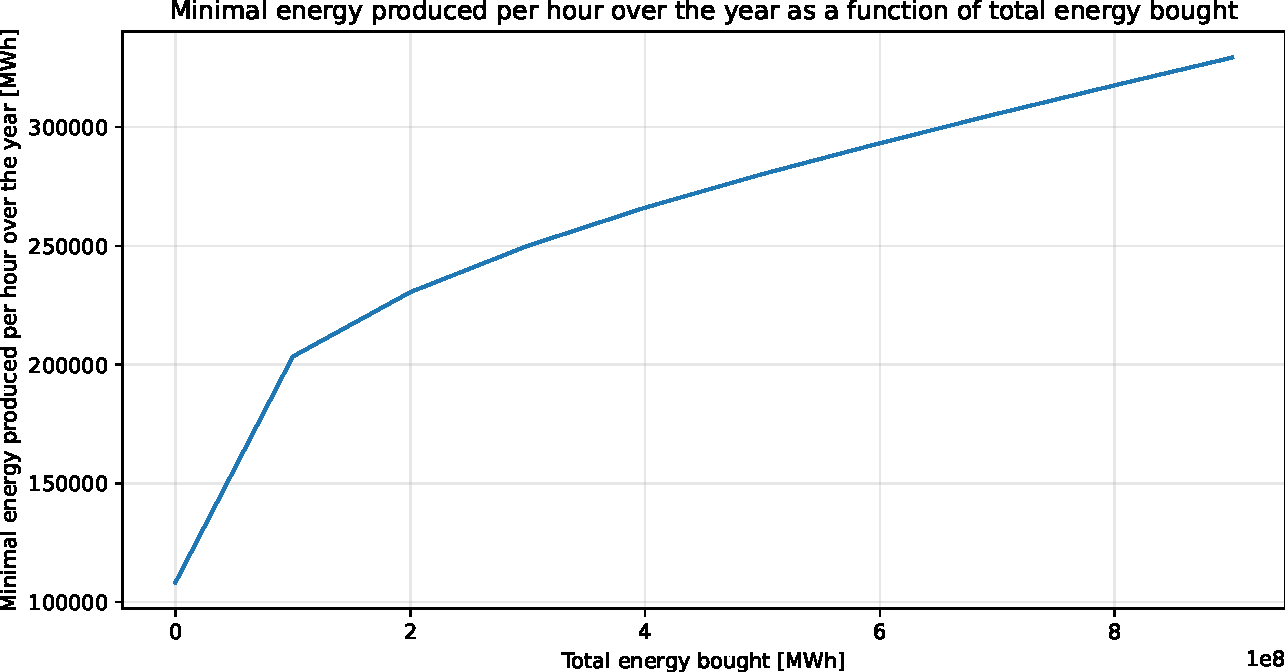
\includegraphics[scale=0.5]{Images/Partie_1/Q2/minimal_energy_produced.pdf}
    \caption{Graphe du minimum de production en fonction de l'énergie maximale achetable}
    \label{fig:minimal_energy_produced_Q2}
\end{figure}
\noindent

Le choix le plus intéressant est en fait l'endroit où la pente est maximale. En effet, en ce point là, acheter une quantité supplémentaire d'énergie amène à une augmentation maximale du minimum de production totale. Le graphe de la pente du graphe ci-dessus est représenté ci-dessous :

\begin{figure}[h!]
    \centering
    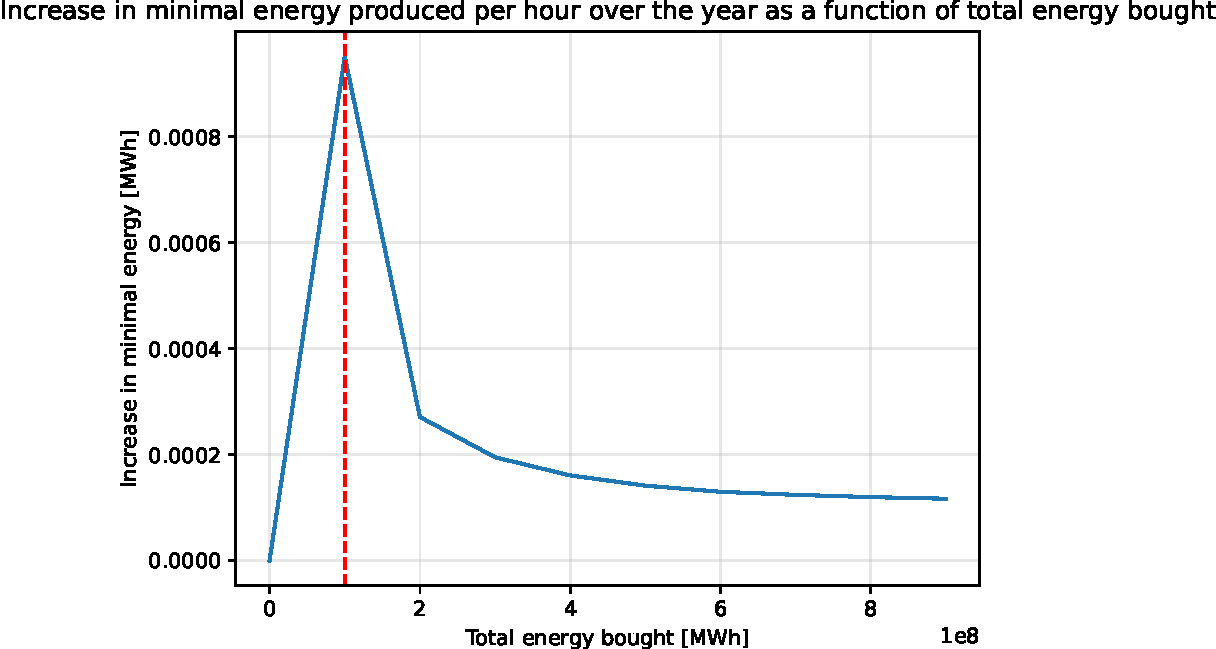
\includegraphics[scale=0.5]{Images/Partie_1/Q2/increase_minimal_energy_produced.pdf}
    \caption{Graphe de la production minimale marginale en fonction de la quantité d'énergie achetable}
    \label{fig:increase_minimal_production_Q2}
\end{figure}

\pagebreak

Nous voyons ici que la production minimale marginale est maximale pour une valeur de $E_{\text{max}} = 1e8 [\mathrm{MWh}]$.
Nous prenons alors cette valeur pour représenter la production totale (donc en prenant compte à la fois l'énergie produite et l'énergie achetée). 

\begin{figure}[ht!]
    \centering
    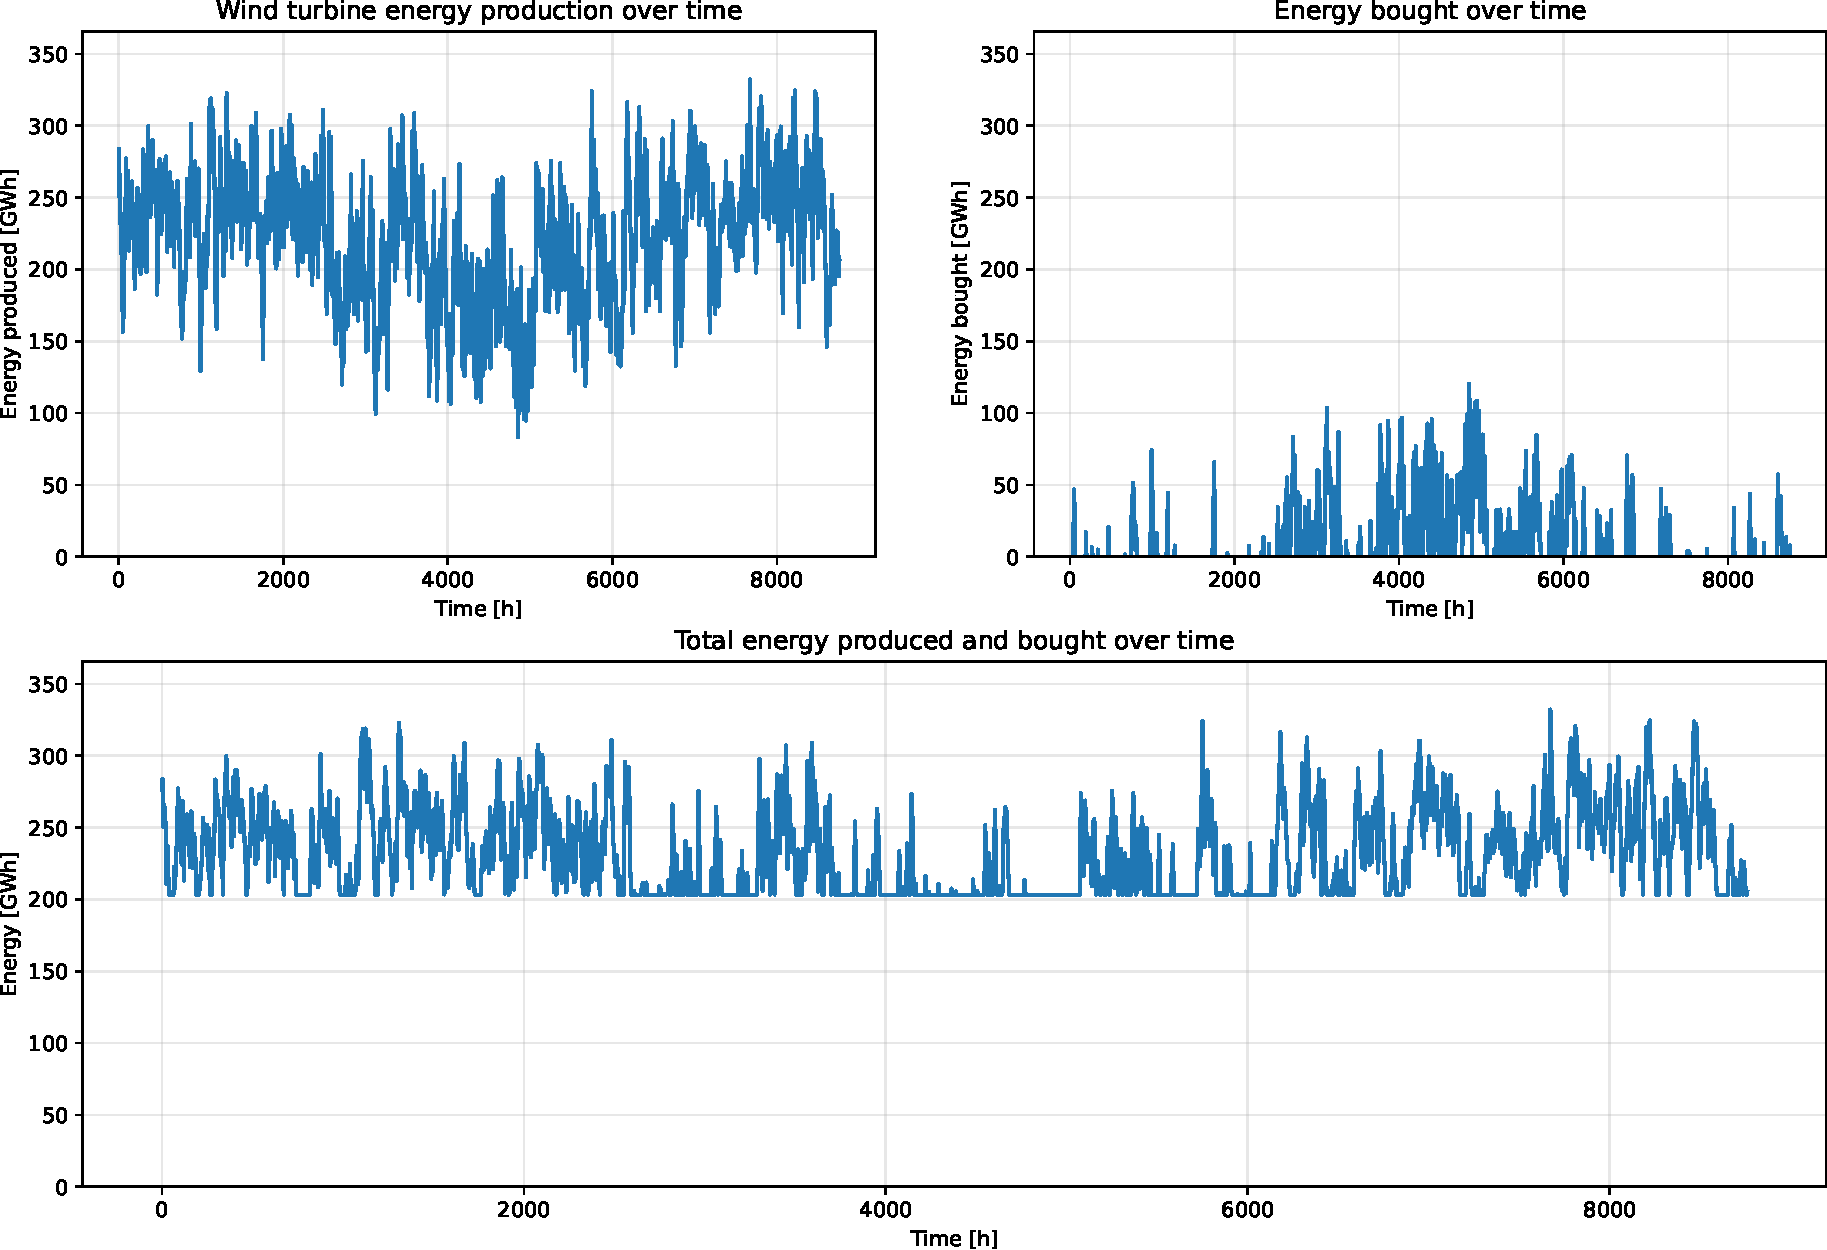
\includegraphics[scale=0.3]{Images/Partie_1/Q2/energy_produced_and_bought.pdf}
    \caption{Graphe de la production totale d'énergie pour $E_{\text{max}} = 1e8 [\mathrm{MWh}]$}
    \label{fig:total_energy_produced_and_bought_Q2}
\end{figure}
Comme nous le voyons sur la figure ci-dessus, la possibilité d'acheter de l'énergie va servir à remonter et à équilibrer les valeurs inférieures de productions d'énergie, d'où le fait que le graphe soit "plat" en-dessous.

\end{document} 